\chapter{Serial Replication in \ak\ }\label{chap_sr}
%The serial replication combinator implements recursive computations and the loop construct with pipeline parallelism.
In this chapter we explain the machinery behind the serial replication in \ak\ and the role of synchronisers in it. We introduce the concept of the forward fixed point for the replication pipeline and show how it is used to organise the output from the infinite chain of replicas. In order to supress the growth of the replica chain, we present the concept of the reverse fixed point and show how it is used to optimise some replicas at the head of the chain.

%First of all, the semantics of AstraKahn on the TPL is described in terms of structures put in place for the coordinator, i.e. a controlling agent, or indeed a group of agents, responsible for progress and communication of the KPN vertices.

    \section{\ak\ Approach to Serial Replication}
The serial replication combinator creates a conceptually infinite number of copies of its operand network, and connects them in a chain. Replication is demand-driven: the replicas are created dynamically. A fresh replica is \emph{inactive}\footnote{More generally, we call a replica inactive when all of its synchronisers are in their start states, none of its channels has messages in them and no box is running}, hence it does not necessarily require significant resouces since \ak\ boxes are stateless and since synchronisers require no resouces in their start state\footnote{When a synchroniser transitions back to the start state, it flushes its store variables}. Indeed the cost of replication is only felt when the replicas are active, which is the case from the time that the first message is received until all messages have left the replica and all its synchronisers have returned to their start states.

In \textsc{S-Net}, the output from a replication pipeline is based on the record subtyping in the type system. The replication combinators in \textsc{S-Net} require the programmer to specify a termination pattern, so that each record that is a subtype of this pattern leaves the replication pipeline throught the output stream.

In \ak\, the output from the replication pipeline is defined using the concept of fixed point. From the mathematical point of view a fixed point of a function is an element of the function's domain that it maps to itself. That is to say, a function $f(x): X \to Y$ has a fixed point at $x_0 \in X$ if $f(x_0) = x_0$. The serial replication combinator implements the computation\footnote{$f^{(n)}(x)$ denotes $\underbrace{f(f(\dots f}_n (x) \dots))$} shown in Fig. \ref{fig:fp}. After the $n$-th replica has processed the message $f^{(n-1)}(x) \neq x_0$ the computation reaches the fixed point $f^{(n)}(x) = x_0$, and the message $x_0$ is sent on to the output channel of the serial replication network $f^{*}$.
\begin{figure}[h!]
\centering
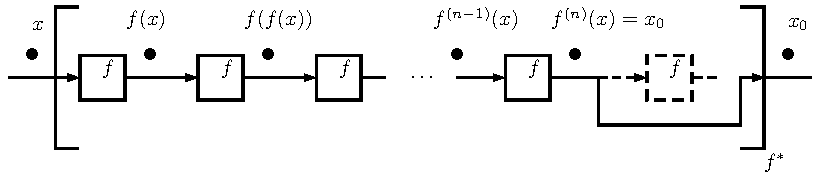
\includegraphics[scale=0.8]{figs/chapter_03_fp.pdf}
\caption{The recursive computation in \ak\ }
\label{fig:fp}
\end{figure}

The number of iterations $n$ needed to reach the fixed point is not known in advance, meaning that in order to utilize the fixed point as shown in Fig. \ref{fig:fp}, \ak\ must be able to detect the fixed point message right at the time it is produced by the $n$-th replica or later. Therefore, similar to \textsc{S-Net}, \ak\ needs to be provided with a pattern that matches all the fixed point messages of the operand network. In \textsc{S-Net}, the serial replication combinator requires this pattern as one of its operands; by contrast, in \ak\ the pattern is required to be deduced from the operand network be compiler analysis.

The chain of replicas grows as the computation progresses, however, in the example in Fig. \ref{fig:fp} the computation is carried out only by a single replica in the tail of the chain. The replicas in the head of the chain have processed the message and are not used anymore. In order to suppress the growth of the chain, \ak\ must detect such replicas and optimise the connection by removing them. Since \ak\ boxes are stateless, an operand network can have a state that is fully defined by the states of its synchronisers. A replica of the operand network can be removed from the chain safely iff the replica is in a state, in which it forwards any message without change, i.e. any message it receives is its fixed point. We will call such a state of the replica a reverse fixed point state.

In the remainder of the chapter we will give formal definitions of a fixed point message and a reverse fixed point state, and will provide algorithms for the \ak\ compiler to detect them. In the sequel, we will call a fixed point message a forward fixed point.


    \section{Forward Fixed Point}
%We will now explain how the pattern to match the fixed point messages can be encoded within the operand network.
Once the computation in a serial replication network has reached the fixed point, newly created replicas are known to transmit fixed point messages without change. \ak\ does not analyse boxes\footnote{Except for the CAL passport generation}, so it can determine about the operand network behaviour only from its synchronisers. Thus, in order for the operand network to be analysable by \ak\, it must contain a path that does not traverse boxes and which may traverse synchronisers. Because a newly created replica is inactive, and hence the synchronisers in it are in their start states, the start states of the synchronisers that belong to the path must have a special transition that sends the message on to the next synchroniser along the path. Since transitions can be conditional on the message content, the fixed point pattern, or rather the fixed point condition, can be present in these special transitions.

%1) synchronisers approach (only detects integer fields like S-Net)
The existence of a forward fixed point requires the operand network to have some topological properties that are formally defined as follows. Consider a network $N$ that has an input and an output channel, both named $x$.

\begin{definition}\label{ffp_def}The network $N$ is said to have a forward fixed point in $x$ if and only if the following requirements are satisfied:
\begin{enumerate}
\item There exists a condition $P(m)$ on the content of the message $m$ received by the network on the input channel $x$ under which it follows a unique non-branching path to the output channel $x$ without traversing any boxes
\item The path\footnote{In the sequel, we will call this path the fixed point path} can traverse synchronisers, but then whenever $P(m)$ is true and the synchroniser is in the start state, it must accept $m$ and transition back to the start state while sending the message $m$ on the path unchanged and without producing any other output
\end{enumerate}
\end{definition}

The condition $P$ may not be unique for each network, and when it is not, the fixed point condition of the network is a disjunction of all such conditions. The condition can also be a tautology, in which case the forward fixed point is called unconditional. When the fixed point path traverses a single synchroniser, the fixed point condition is defined exclusively by the synchroniser transitions that loop around the start state and send on the accepted messages unchanged. When the path traverses several synchronisers, the fixed point condition of the network is a conjunction of the fixed point conditions of these synchronisers. We demonstrate the construction of the fixed point condition with the example operand network $N$ depicted in Fig. \ref{fig:ffp}.

\begin{figure}[h!]
\centering
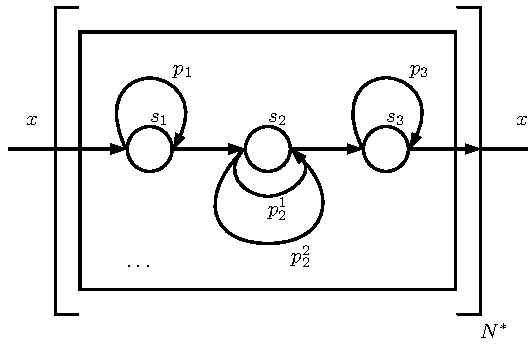
\includegraphics[scale=0.8]{figs/chapter_04_ffp.pdf}
\caption{Forming of the forward fixed point condition of a network}
\label{fig:ffp}
\end{figure}

Apart from all the paths that traverse boxes, the operand network $N$ has a unique path $[s_1, \: s_2, \: s_3]$ that traverses only synchronisers. The synchroniser $s_2$ has two transitions that loop around the start state and send on messages they accept unchanged with the firing conditions $p^{1}_2$ and $p^{2}_2$. A message $m$ is a fixed point for the synchroniser $s_2$ when it satisties any of these conditions, i.e. $p^{1}_2(m) \lor p^{2}_2(m)$ is true. The synchronisers $s_1$ and $s_3$ have fixed point conditions $p_1$ and $p_3$ respectively. Then the fixed point condition of the network $N$ is $p_1 \land (p^{1}_2 \lor p^{2}_2) \land p_3$.

Definition \ref{ffp_def} requires the synchronisers that traverse the fixed point path to transition back to the start state after the fixed point message has been sent to the output channel. This restriction can be relaxed, however, in this case the programmer would have to maintain transitions that check the fixed point condition in every state of each synchroniser along the path.
%or at least in a closed subset of states


    \subsubsection*{Output from the Serial Replication Network}
Now we will clarify how the serial replication network is wired to the rest of the \ak\ application network and how the output is produced. Strictly speaking, the serial replication is not just a wiring pattern since it does not simply wire the replicas of its operand network. It also creates a set of output channels and augments the replicas with some auxiliary synchronisers.

The serial replication $N^{*}$ defines the output channel set $\mathcal{N}_{out}$ as follows:
\begin{equation}
\mathcal{N}_{out} = \{ name(c) \: | \: c \in \mathcal{O} \land fp(c) \}\nonumber
\end{equation}
where $\mathcal{O}$ is the output channel set of $N$ and the predicate $fp(c)$ is true on any channel $c$ that has a forward fixed point. The serial replication creates a set of fresh output channels $\mathcal{O}^{*}$ taking the names from the set $\mathcal{N}_{out}$. A message that is sent to an inactive replica on any channel $c$ with $name(c) \in \mathcal{N}_{out}$ and which satisfies the fixed point condition on that channel is immediately transferred to the identically named output channel from $\mathcal{O}^{*}$. A network in Fig. \ref{fig:ffp_out} demonstrates how the output is produced from the serial replication of a network that has a single input and a single output channel.

\begin{figure}[h!]
\centering
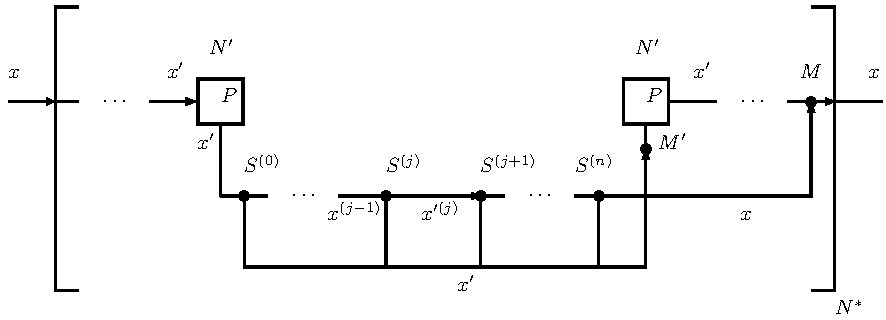
\includegraphics[scale=0.8]{figs/chapter_04_ffp_out.pdf}
\caption{Output from the serial replication network}
\label{fig:ffp_out}
\end{figure}

The operand network $N$ has the fixed point condition $P = \bigvee_{j=0}^{n} p_j$, where $p_j$ is the fixed point condition extracted from the $j$-th synchroniser ($0 \leq j \leq n$) on the fixed point path of $N$. In order to check whether a message $m$ on channel $x'$ satisfies the condition $p_j$, a synchroniser $S^{(j)}$ is inserted before every inactive replica $N'$. If $p_{j}(m)$ is true, the synchroniser sends the message $m$ on to the input channel of the next synchroniser $S^{(j+1)}$ to check whether $p_{j+1}$ is satisfied. Otherwise, the message $m$ is sent to the input channel $x'$ of the next replica of $N$. The listing of the synchroniser $S^{(j)}$, $1 \leq j \leq n-1$ is given in Fig. \ref{ffp:synch_filt}. The synchronisers $S^{(0)}$ and $S^{(n)}$ have the same structure, however, $S^{(0)}$ reads messages from the output channel $x'$ of the previous replica and $S^{(n)}$ sends the message that satisfies $P$ to the output of $N^{*}$. We shall note that for all $j$ for which $p_j = \bigwedge_{i=0}^{k}p^{(i)}_j$ the synchroniser $S^{(j)}$ has $k$ transitions that check the conditions $p^{(i)}_j$.
\begin{figure}[h!]
\begin{lstlisting}[frame=single,mathescape]
synch $S^{(j)}$ ($x'^{(j-1)}$ | $x'^{(j)}$, $x'$)
{
  start {
    on:
      $x'^{(j-1)}$.$p_j$ {
        send this => $x'^{(j)}$;
      }
      $x$.else {
        send this => $x'$;
      }
  }
}
\end{lstlisting}
\caption{The synchroniser $S^{(j)}$}
\label{ffp:synch_filt}
\end{figure}

The merger $M'$ gathers messages that do not satisty the fixed point condition from all synchronisers $S^{(j)}$ between two consecutive replicas of $N$ and forwards them to the input channel of the next replica. The merger $M$ gathers messages that satisfy the fixed point condition $P$ and forwards the messages to the output channel $x$ of the serial replication network $N^{*}$.

%An FPS is a form of replication wiring whereby an infinite chain of replicas is created, connected in series. The connection is denoted as A* for any operand network A and can be thought of as the equivalent of $A^{*} = A'..A'..A'.. \dots$ where $A'$, called the streamlining of the vertex A, is a network that contains A and provides some additional wiring to ensure that each output channel of A? matches an input channel and vice versa. We will dwell on the streamlining procedure a little further down, and at this point only remark that if all output channels of A match its input channels bijectively, A' = A.

    \subsection{Forward Fixed Point Detection}
%    \subsubsection{The Fixed Point Path Search}
%Algorithm that uses extract_ffp, returns the list of all atomic FP conditions for the fixed point message
The existence of a forward fixed point requires the synchronisers that are traversed by the fixed point path to have at least one transition in their start states that accepts the fixed point messages and sends them on unchanged and without producing any other output. Coded in the synchroniser language, the transition that defines the fixed point condition $p$ in channel $x$ is presented in Fig. \ref{ffp:synch_fp}.
\begin{figure}[h!]
\begin{lstlisting}[frame=single,mathescape]
start {
  on:
    x.$p$ {
      send this => out;
    }
  ...
}
\end{lstlisting}
\caption{The start state of a synchroniser that encodes the fixed point condition $p$ in channel $x$}
\label{ffp:synch_fp}
\end{figure}

Note that there exists no other transition on the channel from the start state with the same structure (a single \emph{send} clause). Otherwise, the synchroniser would have the fixed point condition that is the disjunction of conditions in such transitions. The algorithm in Fig. \ref{fig:ffp_extract} checks if a forward fixed point exists on channel $x$ and extracts the fixed point condition from the synchroniser source code. The algorithm supports the renaming of channel $x$ in the synchroniser. Moreover, it may be the case that the transitions that cause a fixed point in the synchronisers send messages to different output channels. The algorithm detects such a situation; however, the branching of the fixed point path is resolved in the context of the whole network.

\begin{figure}[h!]
\noindent\fbox{%
\begin{minipage}{\dimexpr\linewidth-2\fboxsep-2\fboxrule\relax}
\begin{algorithmic}[1]
\Require the abstract syntax tree of the synchroniser program ($synch$), the input label of a channel to test for a forward fixed point ($x$)
\Ensure a dictionary $(a, CondList)$, where $a$ is the output label of the fixed point channel and $CondList$ is the list of atomic fixed point conditions

\Statex
\Function{extract\_fp}{$synch, x$}
  \State $state\gets get the start state tree from synch$

  \State $CondDict\gets nil$
  \Statex
  \For{\textbf{each} \emph{trans in trans\_list}($state$)}
    \If{$get\_port$($trans$) $\neq x$}
      \State \textbf{continue}\Comment{\emph{the transition reads from another channel}}
    \EndIf
    \If{$get\_goto$($trans$) $\neq$ (\tangled{start} $\lor$ $\emptyset$)}
      \State \textbf{continue}\Comment{\emph{the transition does not loop around the state state}}
    \EndIf
    \If{$get\_assign$($trans$) $\neq$ $\emptyset$}
      \State \textbf{continue}
    \EndIf
    
    \State $send\gets get\_send$($trans$)
%    \If{$get\_port$($send$) $\neq$ \tangled{x}}
%      \State \textbf{continue}\Comment{\emph{messages are sent to another channel}}
%    \EndIf 
    \If{$get\_msg$($send$) $\neq$ $this$}
      \State \textbf{continue}
    \EndIf

    \State $cond\gets get\_condition$($trans$)
    \If{$cond$ \emph{is not CondDataMsg} $\lor$ $cond$ \emph{is not CondEmpty}}
      \State \textbf{continue}\Comment{\emph{the condition cannot be a segmentation mark or an} \texttt{.else}}
    \EndIf

    \State $out\_port\gets get\_port$($send$)
    \If{$cond \in CondDict$($out\_port$)}
      \State $CondDict$($out\_port$)$\gets CondDict$($out\_port$) \texttt{..} $cond$
    \Else
      \State $CondDict\gets CondDict$ \texttt{..} ($out\_port$, [$cond$])
    \EndIf

  \EndFor

  \Statex
%  \If{$|keys$($CondDict$)$| \neq 1$}\Comment{\emph{if the number of entries in the dictionary is not 1}}
%    \State \emph{error}
%  \EndIf

%  \If{$CondDict = nil$}
%    \State \emph{error}\Comment{\emph{the synchroniser does not have the fixed point}}
%  \EndIf

  \State \textbf{return} $CondDict$
\EndFunction
\end{algorithmic}
\end{minipage}%
}
\caption{Extracting the fixed point condition from a synchroniser (assumes that channel $x$ is declared as an input and an output channel of the synchroniser)\label{fig:ffp_extract}}
\end{figure}

The fixed point condition of an \ak\ network is formed by the fixed point conditions of its synchronisers that are traversed by the fixed point path. Networks in \ak\ are represented as graphs, thus the fixed point detection is a graph search problem.

A network graph is a directed multigraph because in \ak\ two nodes are not restricted to be connected with only one edge. The graph has four types of nodes, namely a box, a synchroniser, a merger and a network. The fixed point path may traverse nodes of any type except for boxes. If the path traverses a node that is a network, the network must have a forward fixed point as well.

The fixed point detection algorithm (Fig. \ref{fig:ffp_detect}) is based on the depth-first search algorithm with the following considerations:
\begin{itemize}
\item The first and the last nodes of the fixed point path for a particular input channel are known; consequently, only the paths between these two nodes in the graph are traversed

\item If the search encounters a box, the traversed path is rejected

\item If the search encounters a synchroniser, the fixed point condition of the synchroniser is extracted using the function $extract\_fp$ in Fig. \ref{fig:ffp_extract}. If the synchroniser has no fixed point condition, the traversed path is rejected. Otherwise, the search continues only for the successors of the node that were detected by $extract\_fp$

\item If the search encounters a merger, it immediately continues to its only successor

\item If the search encounters a node that encapsulates a network, the fixed point detection is run on the network. If no fixed point path exists for the network, the traversed path is rejected.
\end{itemize}

The fixed point detection algorithm runs only on acyclic networks. The wrap-around wiring makes \ak\ networks cyclic, however, the wrap-around channels cannot carry a fixed point. Therefore, these channels must be filtered before the fixed point detection is run.


%\begin{figure}[h!]
%\noindent\fbox{%
%\begin{minipage}{\dimexpr\linewidth-2\fboxsep-2\fboxrule\relax}
%\begin{algorithmic}[1]
%
%\Require an operand network ($net$), a channel to test for a forward fixed point ($x$)
%\Ensure a set of fixed point conditions on the channel
%
%\Statex
%
%\Function{detect\_ffp}{$net, x$}
%  \State $start\gets$\emph{get a node that has an input port x}
%  \State $end\gets$\emph{get a node that has an output port x}
%  \Statex
%
%  \State \textbf{return} $get\_cond\_list$($net, x, start, end$)\Comment{\emph{Fig. \ref{fig:ffp_get_cond}}}
%%  \If{$|Lists| \neq 1$}
%%    \State \textbf{return} \emph{error}
%%  \EndIf
%%  \State \textbf{return} $Lists$
%\EndFunction
%\end{algorithmic}
%\end{minipage}%
%}
%\caption{A forward fixed point detection in channel $x$ (assumes the network graph is connected)\label{fig:ffp_detect}}
%\end{figure}


\begin{figure}%[h!]
\noindent\fbox{%
\begin{minipage}{\dimexpr\linewidth-2\fboxsep-2\fboxrule\relax}
\begin{algorithmic}[1]
\Require an operand network graph ($graph$), a channel to test for a forward foxed point ($x$), the first and the last node in the fixed point path ($start$, $end$), the list of fixed point conditions gathered along the path ($cond\_list$, optional with the default value $empty\_list$)

\Ensure a set of fixed point conditions on the channel
\Statex

\Function{detect\_ffp}{$graph$, $x$, $start$, $end$, $cond\_list=empty\_list$}
  \If{$start$ \emph{is a box}}
    \State \textbf{return} $empty\_list$
  \EndIf
  \Statex

  \If{$start$ \emph{is a synchroniser}}
    \State $CondDict\gets extract\_fp$($start, x$)
    %What if there're few synch paths and the synch does not have the fixed point???
    \If{$CondDict = nil$}
      \State \textbf{return} $empty\_list$
    \EndIf

    \State $Lists\gets empty\_list$

    \State $cond\_list\gets cond\_list$ \textbf{..} $start\_cond$ %add check if cond already exists in cond_list

    \For{\textbf{each} \emph{succ\_node in succ\_nodes}($start$)}
      \State $out\_port\gets get\_label$($edge$($start, succ\_node$))
      \If{$out\_port \in keys$($CondDict$)}
        \If{$start = end$}
          \State \textbf{return} $cond\_list$
        \EndIf

        \State $NewLists\gets detect\_ffp$($graph, out\_port, succ\_node, end, cond\_list$)

        \For{\emph{new\_list in NewLists}}
          \State $Lists\gets Lists$ \textbf{..} $new\_list$\Comment{\emph{the fixed point path branches if $|Lists|>1$ }}
        \EndFor

      \EndIf
    \EndFor

    \State \textbf{return} $Lists$
  \EndIf
  \Statex

  \If{$start$ \emph{is a merger}}
    \If{$start = end$}
      \State \textbf{return} $cond\_list$
    \EndIf
    \State $out\_port\gets get\_out\_port$($start$)\Comment{a merger has a single output port}
    \State $succ\_node\gets get\_succ\_node$($start$)
    \State \textbf{return} $detect\_ffp$($graph, out\_port, succ\_node, end, cond\_list$)
  \EndIf
  \Statex

% It does not work for 2 consecutive nets in the path
  \If{$start$ \emph{is a network}}
    \State $start\gets$\emph{get a node that has an input port x}
    %run detection for every node that has no successors, must be one path in total
    %\State $end\gets$\emph{get a node that has an output port x} %not x, the channel is unknown

    \State $Lists\gets detect\_ffp$($graph, x, start, end$) %it can be empty_list as well if the network does not have a fixed point, then the path is rejected
    \If{$start = end$}
      
      \State \textbf{return} $cond\_list$ \textbf{..} $Lists$

    \EndIf
    \State \textbf{return} $Lists$
  \EndIf

\EndFunction
\end{algorithmic}
\end{minipage}%
}
\caption{A forward fixed point detection in channel $x$ (assumes the network graph is connected)\label{fig:ffp_detect}}
\end{figure}


    \subsection{Discussion}
The approach we have presented relies on the ability of synchronisers to encode some checks of the message content and perform different actions depending on the result of a check. As the analysis in previous sections shows, the construction of an operand network with a complex fixed point condition can be quite complicated. In order to avoid having to construct complicated operand networks, we provide an additional fixed point detection strategy that relies on a special port wiring primitive $P$ that transmits messages immediately from one port to another without storing them. The programmer now has to make sure that the fixed point messages are detected within the operand network\footnote{It can be done in a box} and sent to $P$. The messages cascade through all the active replicas via a chain of $P$ wires and leave the replication network when they encounter an inactive replica. The example in Fig. \ref{fig:ffp_new} demonstrates how the approach works.

The operand network $A$ in Fig. \ref{fig:ffp_new} has a single input port $x$ and two output ports. The output port $x$ is intended for the messages that proceed to the the next replica of $A$ in the chain, and the output port $x'$ is a auxiliary port for the messages that are supposed to leave the replication pipeline. The serial replication network $A^{*}$ has a single input and a single output port both named $x$. During the compilation, the operand network $A$ is encapsulated into the special network $N$ it as shown in Fig. \ref{fig:ffp_new}. The network $N$ inherits all the ports from $A$ and adds the corresponding input port $x'$. The input and output ports $x'$ of $N$ are connected with the wiring primitive $P$. The output and the input ports $x'$ of the consequent replicas of $N$ are connected with the wiring primitive $P$ as well.
\begin{figure}[h!]
\centering
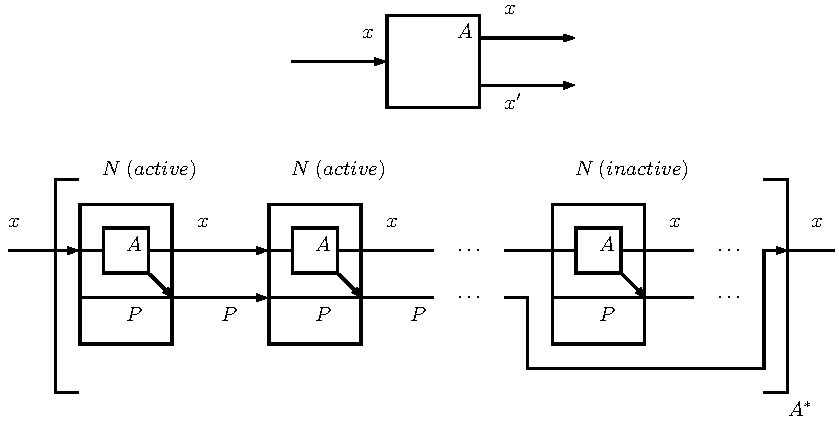
\includegraphics[scale=0.8]{figs/chapter_04_ffp_new.pdf}
\caption{The operand network $A$ (top) and a possible implementation of its serial replication $A^{*}$ (bottom)}
\label{fig:ffp_new}
\end{figure}
A message that $A$ sends to the output port $x'$ cascades through all the active replicas. Once it has reached an inactive replica, the output channel $x$ of $A^{*}$ is dynamically wired to the output port $x'$ of the last active replica of $N$. When an inactive replica becomes active, the port $x'$ is rewired with the input port of this replica using $P$.



%The second approach to the serial replication implementation relies on a merger with variable number of inputs. When a replica of $A$ sends a message to the output port $x'$, a new input channel is created for the merger $M$ and wired to the output port $x'$ of the replica as shown in Fig. \ref{fig:ffp_new_1}. The merger's output port is wired to the output channel $x$ of $A^{*}$.
%\begin{figure}[h]
%\centering
%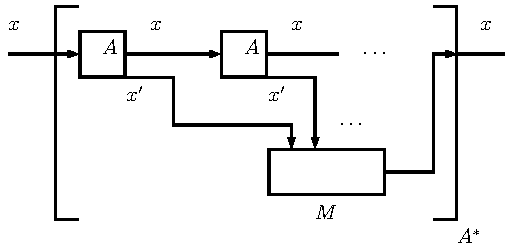
\includegraphics[scale=0.8]{figs/chapter_04_ffp_new_1.pdf}
%\caption{Another possible implementation of the serial replication $A^{*}$}
%\label{fig:ffp_new_1}
%\end{figure}
%
%%The serial replication implements a loop with variable tripcount



    \section{Reverse Fixed Point\label{rfp}}
% TODO: I don't like the reason. Why was the reverse fixed point introduced?
% reverse fixed point is the basic optimisation that preserves growth of the replicas chain.
A reverse fixed point on channel $x$ is a state of a replica, in which it transmits messages from channel $x$ unchanged. A state of a replica is formed by the states of its synchronisers. \ak\ does not analyse boxes and it can determine the operand network behaviour only from its synchronisers. Thus, in order for the operand network to be analysable by \ak\, it must contain a path that does not traverse boxes and which may traverse synchronisers. Every synchroniser that is traversed by the path must have at least one state, in which it accepts a message from channel $x$ unconditionally and sends it on to the next synchroniser along the path without storing or modifying the message.

The existence of a reverse fixed point state requires the operand network to have some topological properties that are formally defined as follows. Consider a network $N$ that has an input and an output channel, both named $x$.

\begin{definition} The network $N$ is said to have a reverse fixed point in $x$ if and only if the following requirements are satisfied:

\begin{enumerate}
\item A unique non-branching path from the input to the output channel $x$ exists that does not traverse any boxes

\item Every synchroniser $S_i$ on the path has a subset of states, which we denote as $s_i$, such that in each of these states every message on the path is immediately transferred without being changed or stored, causing the synchroniser to remain in the same state\footnote{We shall note that the values of any state variables form a part of the synchroniser state}. In a state from $s_i$ the synchroniser $S_i$ may still be sensitive to other input channels, as long as this does not, under any circumstances, cause a transition to a state outside $s_i$
\end{enumerate}
The network $N$ is said to be in a reverse fixed point state on channel $x$ when each $S_i$ is in a state that belongs to its $s_i$.
\end{definition}



%%%%%%%%%%%%%%%%%%%%%%%%%%%%%%%%%%%%%%%
%%%%%%%%%
%%  Motivation for the reverse fixpoint
%%%%%%%%%
%The reverse fix-point is defined to unify backslash \ combinatior and the star in terms of their functionality, which was never done in S-Net(TODO which patterns??). The intention is that they only differ in the pressure propagation strategy. The backslash creates no pressure (TODO why??) in its looped channel, and the start mantains and propagates the pressure in channels between instanses.
%
% probably a picture
%
% backslash (* is the synchroniser)
%      _________
%    \|/ _____  |
% ____*_|     |_|
%       |_____|
%
%
% Star with the reverse fix point
%        __________________
%      _|___________       |
%    _|______       |      |
%   |    __ \|/ __ \|/ __ \|/ __
% --*---|__|-*-|__|-*-|__|-*-|__|-- ...
%
%
%The reverse fix point is more the way to write code. It is the way to program a loop dependency, when the result of the iteration depends not only on the result of the previous iteration but on the new incoming data. The difference with backslash is in the pressure propagation.
%
%If you want the feature, you must define a closed set of translating states in every synchroniser on the fp path.
%%%%%%%%%%%%%%%%%%%%%%%%%%%%%%%%%%%%%%%


    \subsubsection*{Rewiring of the Reverse Fixed Point}
The reverse fixed point optimises an input connection that has to cascade through the chain to a replica that is ready to accept the data.

The operand network $N$ in Fig. \ref{fig:rfp_wiring} has two input and two output channels $x$ and $y$. Any input channel $x$ wired to an active replica of $N$ that transitions to a reverse fixed point state on that channel is disconnected from the replica and dynamically rewired to the input port $x$ of the next replica in the chain.
\begin{figure}[h!]
\centering
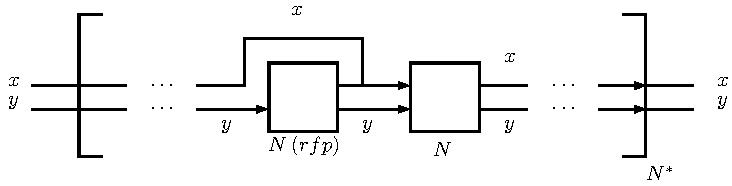
\includegraphics[scale=0.8]{figs/chapter_04_rfp_wiring.pdf}
\caption{Rewiring of a Reverse Fixed Point replica $N\:(rfp)$ on channel $x$}
\label{fig:rfp_wiring}
\end{figure}

If a replica transitions to a reverse fixed point state on every one of its input channels, no box is running and the channels are empty, the replica is removed from the chain.



    \subsection{Reverse Fixed Point Detection\label{rfp_detect}}
The existence of a reverse fixed point on channel $x$ requires the synchronisers that are traversed by the fixed point path to have at least one state, in which they unconditionally accept messages from that channel, send them on along the path unchanged and then transition back to the same state. A synchroniser that is in the reverse fixed point state never transitions from it. Coded in the synchroniser language, a transition that makes a state of a synchroniser the reverse fixed point state on channel $x$ is given in Fig. \ref{fig:rfp_trans}.
\begin{figure}[h!]
\begin{lstlisting}[frame=single,mathescape]
s {
  on:
    x {
      send this => out;
      goto s;
    }
  ...
}
\end{lstlisting}
\caption{The reverse fixed point state $s$ of a synchroniser on channel $x$}
\label{fig:rfp_trans}
\end{figure}

Note that all other transitions from state $s$ must come back to state $s$. As long as they do they can even change the state variables of the synchroniser; the reverse fixed point is unconditional and it exists for any values of the store variables.

The algorithm in Fig. \ref{fig:rfp_extract} checks if a reverse fixed point exists on channel $x$ and extracts all fixed point states from the synchroniser source code. The algorithm is designed to work with the detection algorithm in Fig. \ref{fig:ffp_detect}.
%The algorithm supports the renaming of the fixed point channel in the synchroniser. Similarly, the branching of the fixed point path is resolved in the context of the whole network.

\begin{figure}[h!]
\noindent\fbox{%
\begin{minipage}{\dimexpr\linewidth-2\fboxsep-2\fboxrule\relax}
\begin{algorithmic}[1]
\Require the abstract syntax tree of the synchroniser program ($synch$), the input label of a channel to test for a forward fixed point ($x$)
\Ensure a dictionary $(a, StateList)$, where $a$ is the output label of the fixed point channel and $StateList$ is the list of the reverse fixed point states of the synchroniser

\Statex
\Function{extract\_fp}{$synch, x$}
  \State $rfp\_states\gets$ \emph{all states from} $synch$ \emph{that have transitions like in Fig. \ref{fig:rfp_trans}}
  \State $result\gets \emptyset$
  \Statex

  \While{$rfp\_states \neq result$}
    \If{$result \neq \emptyset$}
      \State $rfp\_states\gets result$
      \State $result\gets \emptyset$
    \EndIf

    \For{\textbf{each} $state$ \emph{in} $rfp\_states$}
      \State $gotos\gets$ \emph{all destination states in} $state$
      \If{$gotos \setminus rfp\_states = \emptyset$}
        \State $result\gets result \cup state$
      \EndIf
    \EndFor

    \If{$result = \emptyset$}
      \State \textbf{return} \emph{no reverse fixed point state found}
    \EndIf

  \EndWhile
  \Statex

  \State $StateDict\gets nil$
  \For{\textbf{each} $state$ in $result$}
    \State $rfp\_out\gets$ \emph{output channel labels of the RPF transitions from} $state$
    \For{\textbf{each} $out$ \emph{in} $rfp\_out$}
      \If{$out \notin StateDict$}
        \State $StateDict$($out$)$\gets state$
      \Else
        \State $StateDict$($out$)$\gets StateDict$($out$) \textbf{..} $state$
      \EndIf
    \EndFor
  \EndFor

  \Statex
  \State \textbf{return} $StateDict$
\EndFunction
\end{algorithmic}
\end{minipage}%
}
\caption{Extracting the reverse fixed point from a synchroniser (assumes that channel $x$ is declared as an input and an output channel of the synchroniser)\label{fig:rfp_extract}}
\end{figure}

